\chapter{Evaluation}
\label{chap_eval}

In Chapter 3, Outlining the process of story-centric brainstorming and collaboration, I concluded that the process works toward the goals mentioned in the introduction section. Nonprofits have had valuable insights by working with makers, they have learned about their unique skill sets and collaborated towards solutions. Makers, in turn, practiced their skill sets and gained confidence in their abilities.

In this chapter, I focus on evaluating the move from ``real life'' collaborations to online collaborations using the newly built \textit{This is How} platform. I start by evaluating the video medium itself and then examine the platform by means of comparison to the test cases presented in Chapter 3.

\section{Video production} 
\label{video_production}

As a tool for evaluation, I produced two video stories. The first, showing the \textit{Mother's Milk Bank Northeast}, was a short one minute video capturing the different steps the milk processing process. It was shot with amateur equipment and edited by myself. The second, capturing the story of \textit{Cradles to Crayons}, was a two minute video shot and edited by Paula Aguilera, Multimedia Producer at the MIT Media Lab, with professional equipment. Our guidelines for creating these videos: 

\begin{itemize}
   \item Provide a general overview of the operation, one that conveys its importance and complexities but can be understood by a non-technical person.   
   \item Discuss the processes employed by the nonprofit while mentioning challenges, constraints and technical details. These details should be superficial enough in order not to be cumbersome for the less technical viewer yet allow for makers who are interested in these topics to ask questions and initiate a discussion.
   \item The audio track should be a voice narration and the image should correlate with the physical items being discussed in the narration, to the extent possible. 
   \item Keep it short - under 2 minutes. 
\end{itemize}

\section {Video - Sanity Check}

Before building \textit{This is How}, as a preliminary study, I tested the effectiveness of video as a medium with a group of makers. I built a static website, containing the video story of Cradles to Crayons, along with three shorter challenges videos. This webpage was shown to a group of makers from the South End Technology Center (SETC) in Boston.

\begin{figure}[thpb]
   \centering
   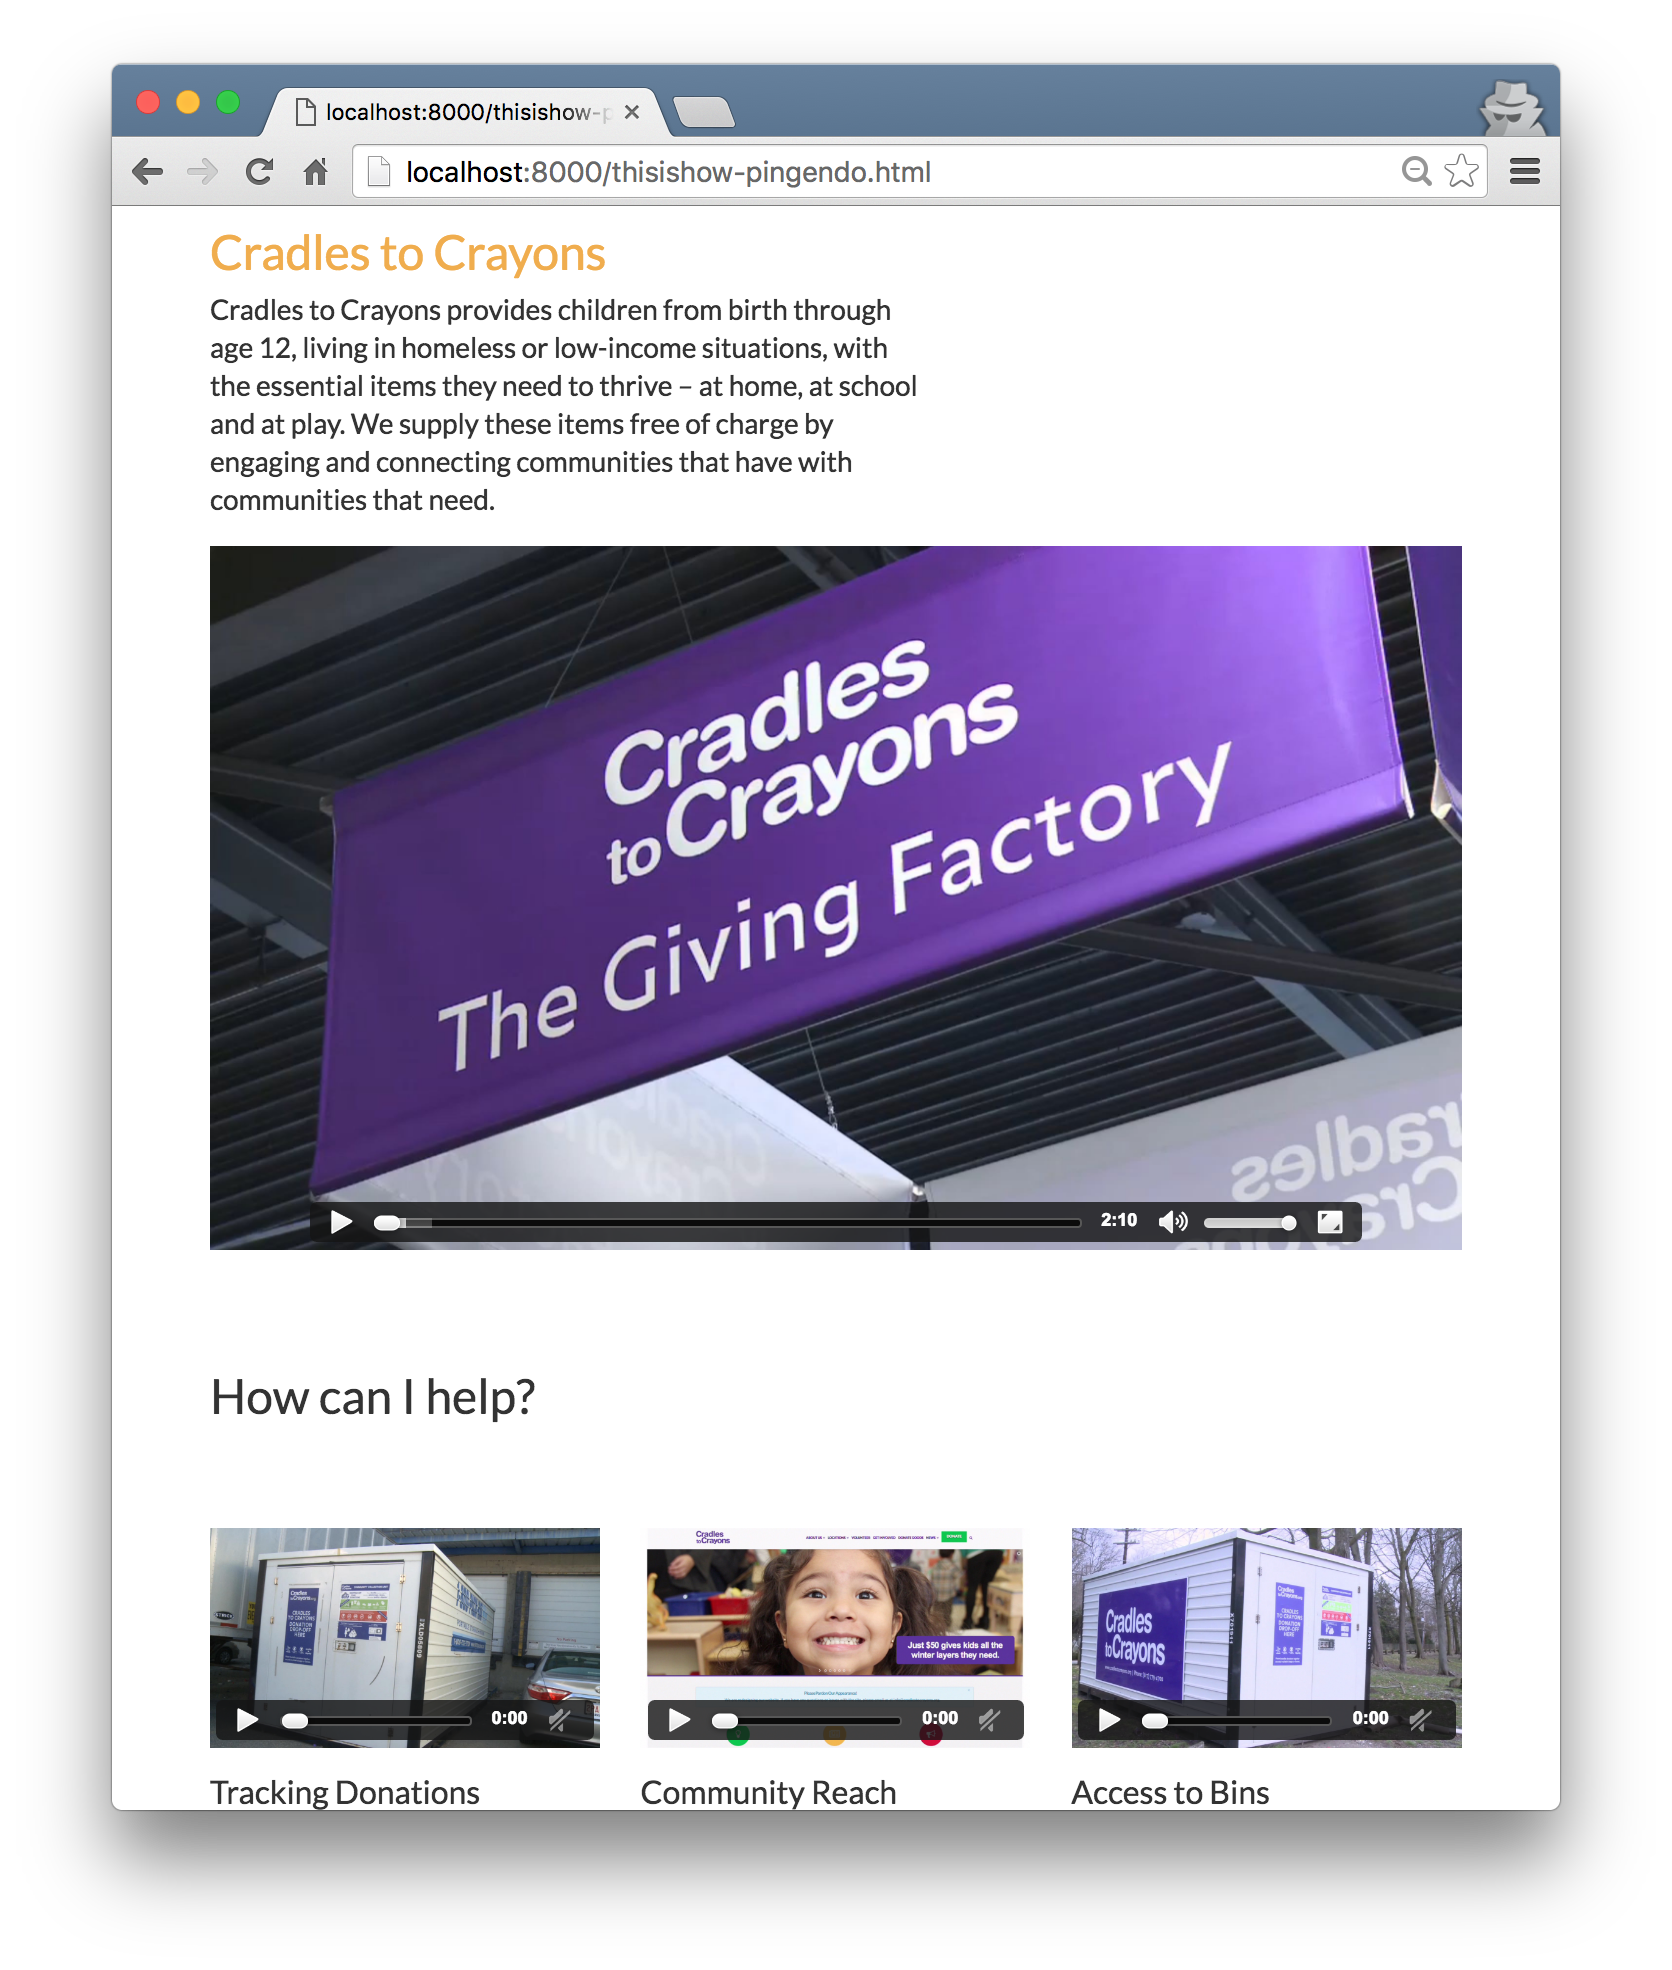
\includegraphics[width=\textwidth]{figures/thisishow-mockup.png}
   \caption{This is How - Early mockup}
   \label{fig_thisishow_mockup}
\end{figure}

The SETC is a maker space, a part of the global fablab \cite{fablab} network of maker­spaces. SETC is unique in that it is operated by high school students. The students take part in a program called ``Learn to Teach, Teach to Learn'' in which they both learn fabrication skills and pass them on to the community and other students throughout the year. During the summer, the students work on projects that utilize the different skills they've learned.

I joined one of the weekly classes these students attended and presented the Cradles to Crayons story through the web page mentioned above. The Video story was shown along with another short video that provides extra details about a specific challenge faced by the organization. I myself did not add any information beyond the videos shown. I then opened a discussion by asking the students what they learned about the nonprofit and how they could utilize their skills to help it. Although some of the students already knew about the nonprofit, they were still surprised to learn about the complexities of running its operations. They then expressed interest in working on projects that might help in dealing with the challenges faced by the nonprofit. These project proposals were surprisingly similar to the ones proposed by other makers in the on site visit described in Chapter 3.

\begin{figure}[thpb]
   \centering
   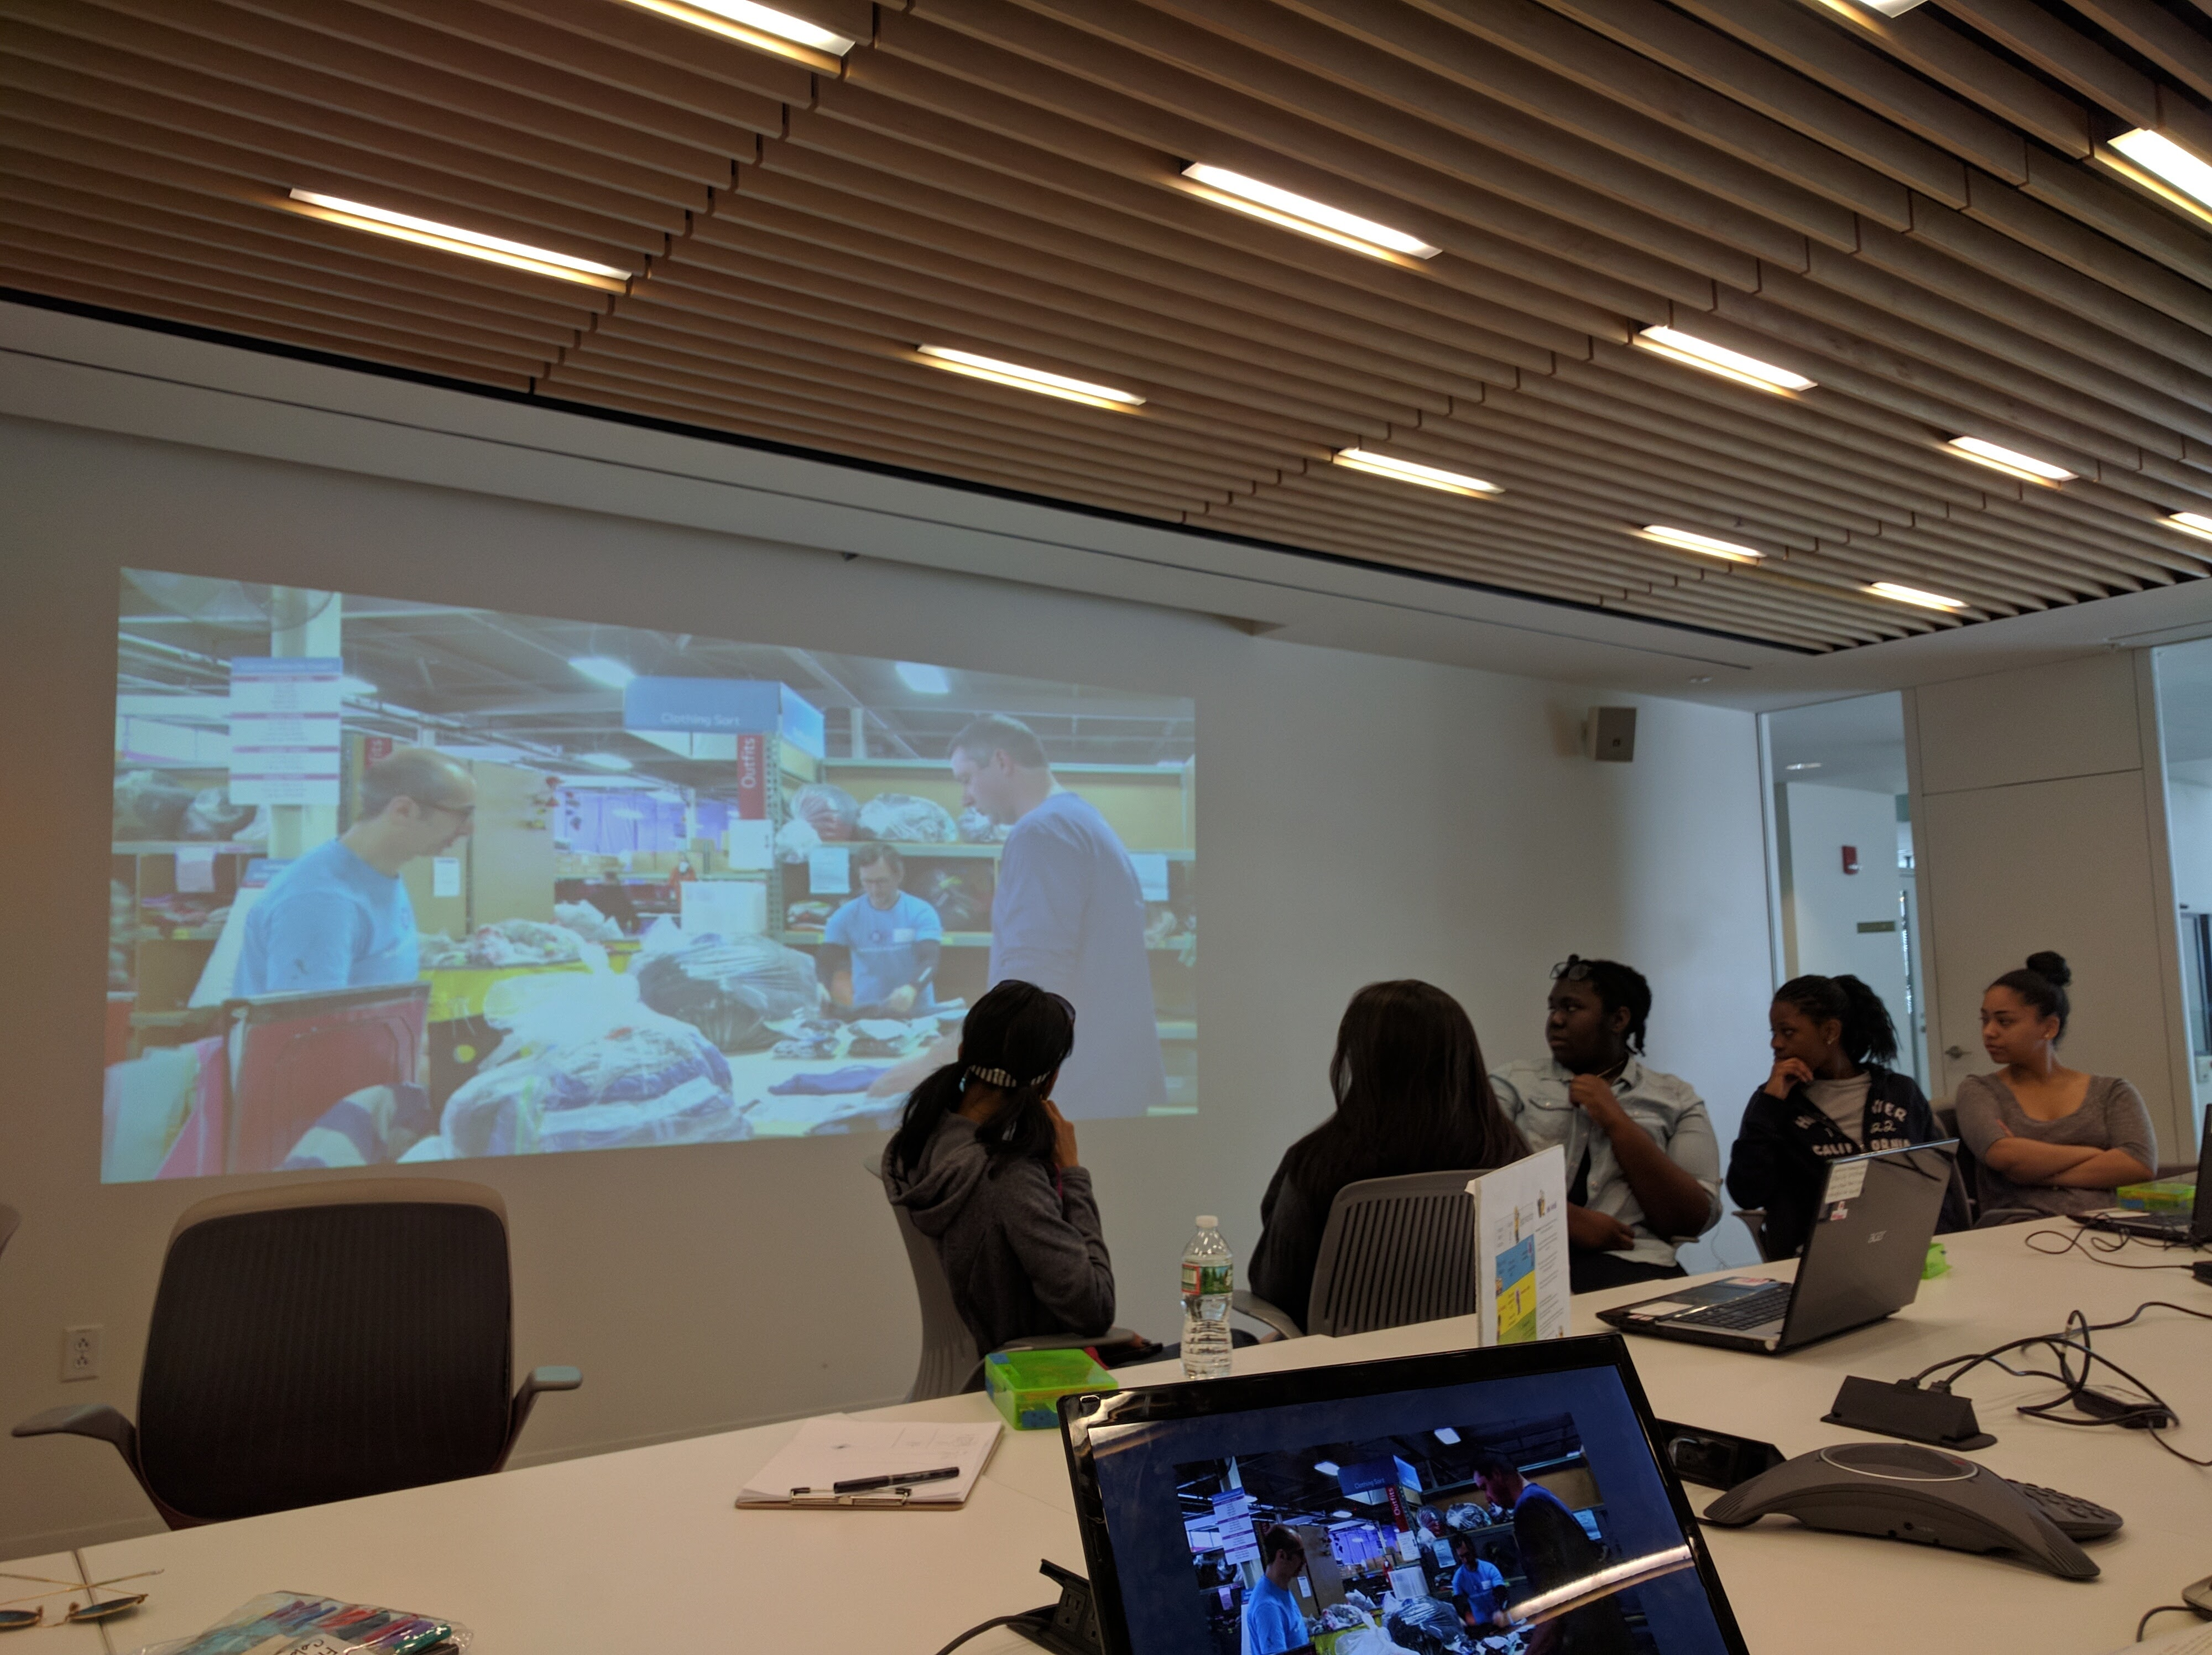
\includegraphics[width=\textwidth]{figures/learn2teach.jpg}
   \caption{Presenting the Cradles to Crayons story at a \textit{Learn to Teach, Teach to Learn} session}
   \label{fig_setc}
\end{figure}

Later that day, Susan Klimczak, who runs the program, sent me an email regarding the visit which included the following:

\begin{quotation}

``When we did feedback, 5 of the youth talked about how meaningful it was to have you come in \& do the cradles to crayons! They said that it would be very valuable to have you come in regularly to present real community issues that need to be solved.''

\end{quotation}

Even without the components of interactivity and collaboration towards a solution, it was clear that the video achieved two important goals. First, it managed to raise awareness for the nonprofit, and second, it empowered the makers by providing a real world example of the value of their skills and inspire them to apply them in new ways.

\section{User Experience Evaluation}

I conducted user-tests with all three nonprofits mentioned in Chapter 3 as well as three makers who participated in some sort of collaboration with them. The evaluation centered around an interactive demonstration, it started from the main story page, including commenting and idea pads, and then moved on to browsing and story creation. 

Per step, the user was requested to comment on ease of use based on their personal experience and compare with the equivalent step in their experience in previous collaborations. 

\subsection{Story Comments System}

The subjects were shown an existing video story with comments, and comment replies, both in the form of text and video.

There was a unanimous agreement between subjects that once an existing comment in the video appears, the timeline based discussion is self explanatory. Some of the interviewees stated that clicking on a comment to open the reply-to-comment system is not intuitive, However, once having seen it, the options to reply by text or video are self explanatory and valuable.

Makers and nonprofits alike have stated that this step seems to be true to the purpose of interactive exploration, as experienced in their collaborations. Some subjects thought the asynchronous nature of the online discussion has more potential than real life interactions because it gives the parties a chance to think about their replies. Others stated the opposite, that the asynchronous nature removes a sense of urgency which exists in real-life discussion and drives it. 

\subsection{Story Creation}

This step focused on the nonprofits, being the story creators, which all stated that the form and mechanics of uploading a file were straightforward and self explanatory, including the usage of tags as keywords. 

This step also served as a trigger for discussion regarding the feasibility of producing a compelling video story. The two smaller nonprofits stated that they believe it's within their reach to produce such a video while C2C, the largest and most established one, raised a concern regarding video quality. All media released to the public domain by them must be vetted to comply with the organization's public relation's team which has high standards.

This was a surprise and the exact opposite of what I expected. I expected the small nonprofits to be hesitant about producing a video, due to their lack of resources, and the bigger one, having a dedicated public relations department, to view this as a manageable task.

\subsection{Idea Pad}

The subjects were shown an Idea Pad with existing ideas regarding the same story as the previous section. Some of these ideas have already featured a number of comments and inputs from various other users.

All the nonprofits stated that it is hard to evaluate without real usage although it seems to be straightforward and fits the process of brainstorming. C2C, the larger nonprofit and also the most aware of public relations, was worried that non-makers who visit the page, will not understand the goal of the idea pad.   

Two of the makers appreciated the lack of structure in the pad as a tool for free form brainstorming while the third was worried of the exact opposite, that the lack of structure does not accommodate the relationships between ideas.

\subsection{Browsing}

The subjects were shown the main page along with the option to filter by tags.

Nonprofits were neutral in their response while makers expressed a concern about scalability, and that the page design may not ideally accommodate large numbers of videos, including the lack of a free form search option.

\subsection{Overall User Experience}
The subjects were asked about the user experience in general and how well it can facilitate story-centric brainstorming and ideation, according to their experience.  

Makers and nonprofits alike have stated that in general the user interface provides a concise and self explanatory experience. The novel components, including the commenting system and the idea pad, became clear once they saw them populated with data.     

All subjects were excited about \textit{This is How} and its potential in fostering collaborations between makers and nonprofits. However, nonprofits were concerned about the discoverability of their Story, they were not convinced that they can attract makers to collaborate with them.     

\subsection{Conclusion}

The results presented in this section are encouraging. They show that the user experience, according to the relevant stakeholders, presents a viable alternative to ``real life'' collaborations.

The commenting system and the idea pad, which are non standard user interface components, proved to be self explanatory when populated with existing data. This can be addressed in two ways: First, when officially launching this platform, to already have curated content that allows users to learn. Second, introducing a first time usage tutorial which covers the basics of commenting and collaborating on ideas.

The weakest aspect of \textit{This is How} in it's current form appears to be discovery. This is obvious from the feedback of the makers regarding browsing and from the nonprofits' general concern about discoverability. Inherent to the act of discovering is the existence of a large corpus of data. It is hard to predict how systems act at scale, especially when that scale represents the behavior of human beings. The only viable solution is to observe the system as it grows and make changes accordingly.